\section[Лабораторная работа №1]{Лабораторная работа №1. \\
Знакомство с виртуализацией. Система виртуализации Oracle VM VirtualBox}

\textbf{Цель работы:} ознакомиться с основными понятиями виртуализации, системой виртуализации VirtualBox, научиться настраивать виртуальную машину (ВМ), совершать простейшие операции с ней, устанавливать операционную систему на ВМ.

\subsection{Теоретические основы виртуализации}

Виртуализация "--- абстракция вычислительных ресурсов и предоставление пользователю системы, которая инкапсулирует (скрывает в себе) собственную реализацию.

Виртуализацию можно использовать в \cite{sevconf2014}:
\begin{itemize}
    \item консолидации серверов (позволяет мигрировать с физических серверов на виртуальные, тем самым увеличивается коэффициент использования аппаратуры, что позволяет существенно сэкономить на аппаратуре, электроэнергии и обслуживании);
    \item разработке и тестировании приложений (возможность одновременно запускать несколько различных ОС, это удобно при разработке кроссплатформенного ПО, тем самым значительно повышается качество, скорость разработки и тестирования приложений);
    \item бизнесе (использование виртуализации в бизнесе растет с каждым днем и постоянно находятся новые способы применения этой технологии, например, возможность безболезненно сделать снапшот\footnote{Снапшот (англ. snapshot) "--- снимок состояния ВМ в определенный момент времени. Сюда входят настройки ВМ, содержимое памяти и дисков} и быстро восстановить систему в случае сбоя);
    \item организации виртуальных рабочих станций (так называемых <<тонких клиентов>>\footnote{Тонкий клиент (англ. thin client) "--- бездисковый компьютер-клиент в сетях с клиент-серверной или терминальной архитектурой, который переносит все или большую часть задач по обработке информации на сервер}).
\end{itemize}

Общая схема взаимодействия виртуализации с аппаратурой и программным обеспечением (ПО) представлена на рис.~\ref{pic:virt_scheme}.
\begin{figure}[ht]
    \centering
	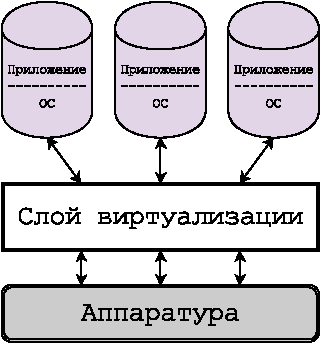
\includegraphics[width=0.35\linewidth]{virt_scheme}
	\caption{Схема взаимодействия виртуализации с аппаратурой и ПО}\label{pic:virt_scheme}
\end{figure}

Взаимодействие приложений и операционной системы (ОС) с аппаратным обеспечением осуществляется через абстрагированный слой виртуализации.

Существует несколько подходов организации виртуализации:
\begin{itemize}
    \item эмуляция оборудования (QEMU, Bochs, Dynamips);
    \item полная виртуализация (KVM, HyperV, VirtualBox);
    \item паравиртуализация (Xen, L4, Trango);
    \item виртуализация уровня ОС (LXC, OpenVZ, Jails, Solaris Zones).
\end{itemize}

Эмуляция аппаратных средств является одним из самых сложных методов виртуализации (рис.~\ref{pic:emulation}).
В то же время главной проблемой при эмуляции аппаратных средств является низкая скорость работы, в связи с тем, что каждая команда моделируется на основных аппаратных средствах.
В эмуляции оборудования используется механизм динамической трансляции, то есть каждая из инструкций эмулируемой платформы заменяется на заранее подготовленный фрагмент инструкций физического процессора.
\begin{figure}[ht]
    \centering
	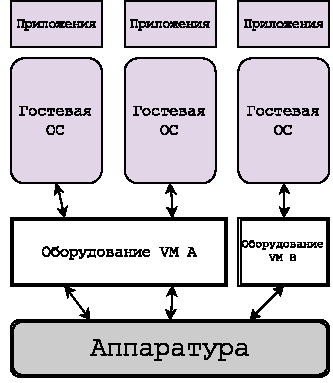
\includegraphics[width=0.35\linewidth]{emulation.pdf}
	\caption{Эмуляция оборудования моделирует аппаратные средства}\label{pic:emulation}
\end{figure}

В случае полной виртуализации поверх уже установленной ОС, устанавливается программа-гипервизор\footnote{Гипервизор (англ. hypervisor)"--- программа или аппаратная схема, позволяющая одновременное, параллельное выполнение нескольких ОС на одном и том же компьютере, обеспечивает изоляцию операционных систем друг от друга}, которая осуществляет взаимосвязь между гостевыми ОС и хост-компьютером (рис.~\ref{pic:full_virt}).
\begin{figure}[ht]
    \centering
	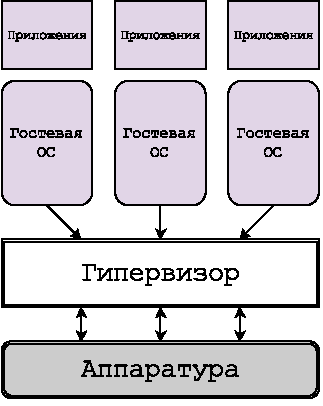
\includegraphics[width=0.35\linewidth]{full_virt}
	\caption{Полная виртуализация использует гипервизор}\label{pic:full_virt}
\end{figure}

Преимуществом технологии полной виртуализации является установка различных ОС, а недостатком "--- меньшая производительность, за счет накладных расходов на гипервизор, а также понижение скорости работы с подсистемой ввода/вывода из-за необходимости изоляции.

Паравиртуализация имеет некоторые сходства с полной виртуализацией.
В данном методе также используется гипервизор для разделения доступа к аппаратуре, но объединяется код, касающийся виртуализации, в ОС \cite{virtuallinux} (рис.~\ref{pic:paravirt}).
\begin{figure}[ht]
    \centering
	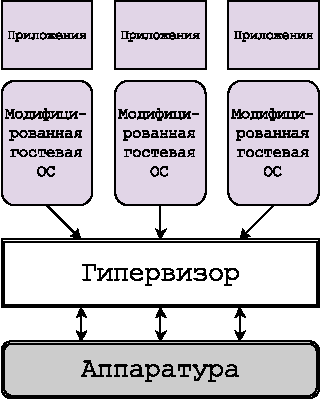
\includegraphics[width=0.35\linewidth]{paravirt}
	\caption{Паравиртуализация разделяет процесс с гостевой ОС}\label{pic:paravirt}
\end{figure}

Недостатком паравиртуализации является необходимость изменения гостевой ОС для гипервизора, однако таким образом гораздо увеличивается производительность.

Виртуализация уровня операционной системы не нуждается в гипервизоре.
Для ее работы необходимо модифицированное ядро на хост-системе с набором патчей и утилит для управления контейнерами\footnote{Контейнер или VPS/VDS (англ. Virtual Private/Dedicated Server) "--- виртуальный выделенный сервер, эмулирует работу физического сервера} (рис.~\ref{pic:cont_virt}).
\begin{figure}[ht]
    \centering
	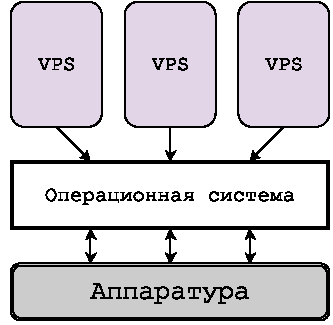
\includegraphics[width=0.35\linewidth]{cont_virt}
	\caption{Виртуализация уровня ОС изолирует серверы}\label{pic:cont_virt}
\end{figure}

За счет того, что контейнер напрямую взаимодействует с ядром, а не через гипервизор, обеспечивается максимальное быстродействие. Но, так как для всех контейнеров используется общее ядро, то нет возможности использовать разные ОС в контейнерах.

Oracle VM VirtualBox "--- система виртуализации, разработанная компанией Innotek в 2007 году, позже приобретена компанией Sun Microsystems.
Ключевыми возможностями системы является кроссплатформенность, наличие графического интерфейса, локализация, поддержка аппаратной виртуализации, экспериментальное 3D-ускорение, поддержка различных образов жестких дисков, возможность установки дополнений гостевой ОС, например для корректной работы проброшенных USB-устройств или возможности изменения разрешения рабочего стола гостевой ОС.

На рис.~\ref{pic:win7-centos} изображен пример одновременной работы двух виртуальных машин (Windows 7 и CentOS 7).
\begin{figure}[ht]
    \centering
	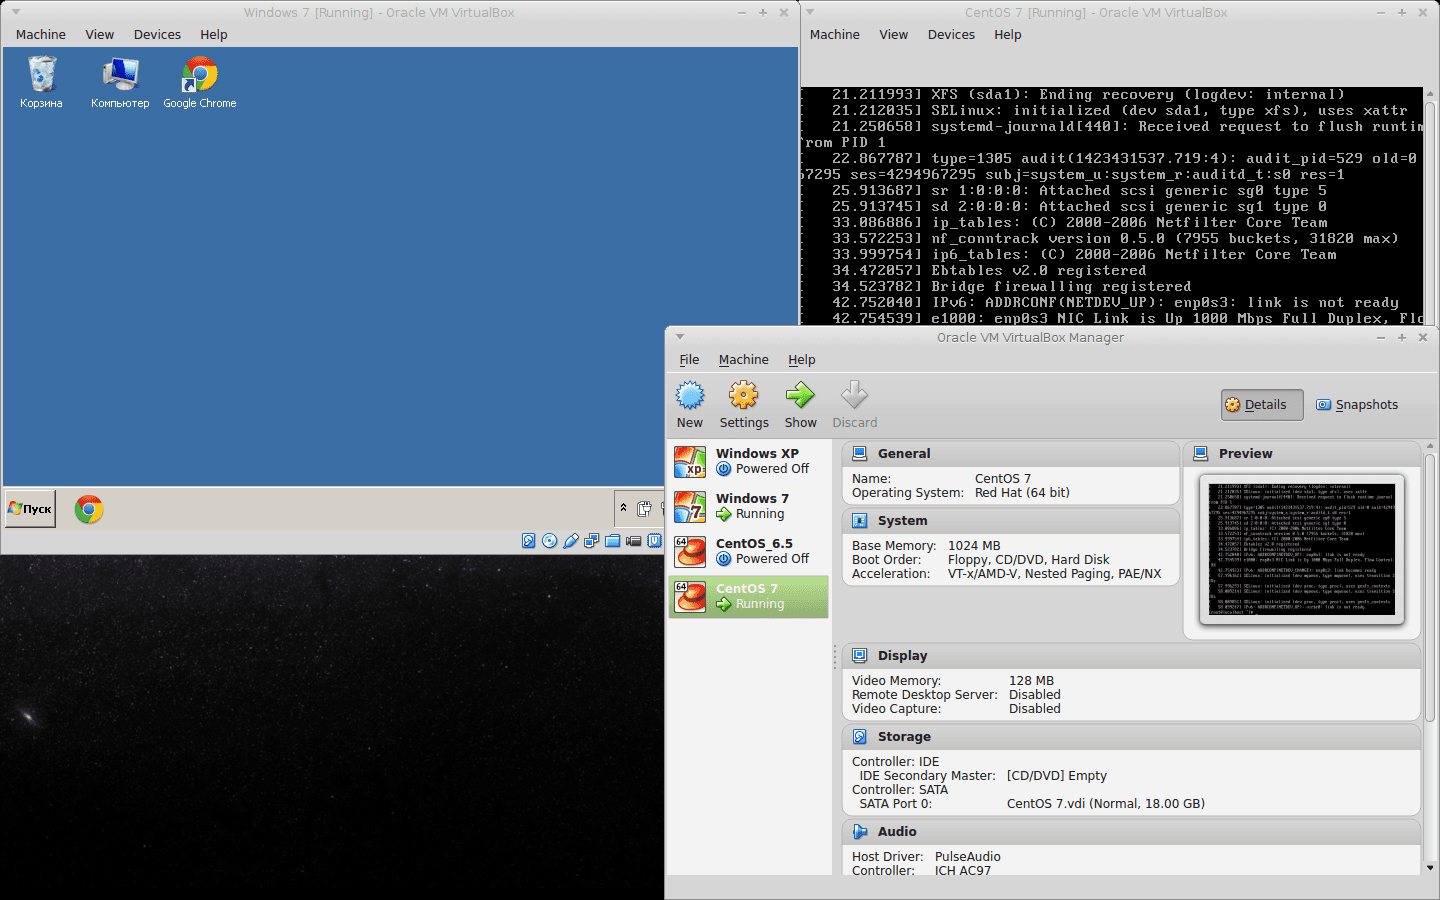
\includegraphics[width=\linewidth]{win7-centos}
	\caption{Пример одновременной работы Windows 7 и CentOS 7}\label{pic:win7-centos}
\end{figure}

\subsection{Порядок выполнения работы}

\begin{enumerate}
    \item Скачать\footnote{\url{https://www.virtualbox.org/wiki/Downloads}} и установить Oracle VM VirtualBox;
    \item Изучить интерфейс программы и создать\footnote{Пример создания виртуальной машины описан в прил.~\ref{pril:a}} первую виртуальную машину на основе образа Debian GNU/Linux\footnote{\url{https://www.debian.org/distrib/}};
    \item Подключить к виртуальной машине ранее скачанный образ Debian GNU/Linux;
    \item Загрузиться с подключенного образа и установить\footnote{Процесс установки Debian GNU/Linux описан в прил.~\ref{pril:b}} дистрибутив на виртуальный жесткий диск;
    \item Во время установки дистрибутива необходимо будет задать пароль суперпользователя, пароль: \texttt{toor}, пароль для локального пользователя можно задать произвольный, но лучше его запомнить;
    \item С помощью команд \texttt{free}, \texttt{df}\footnote{Команды \texttt{free} и \texttt{df} используют ключ \texttt{-h} для показа информации в удобном для человека виде}, \texttt{cat /proc/cpuinfo}, \texttt{ifconfig}, посмотреть параметры виртуальной машины;
    \item С помощью команды \texttt{ping} проверить доступность виртуальной машины в сети как с хост-ноды, так и с других компьютеров сети;
    \item С помощью SSH-клиента (например Putty\footnote{\url{http://www.chiark.greenend.org.uk/~sgtatham/putty/}}) подключиться по SSH к виртуальной машине.
\end{enumerate}

\subsection{Контрольные вопросы}
\begin{enumerate}
    \item Какие типы виртуализации Вы знаете? В чем между ними различия?
    \item К какому типу виртуализации относится система Oracle VM VirtualBox?
    \item Как может использовать виртуализацию в работе веб-программист, системный администратор, сетевой инженер?
    \item В чем состоит основное преимущество и недостаток полной виртуализации от контейнерной?
    \item В чем различие между режимами сети NAT и сетевой мост (Network Bridge)?
\end{enumerate}

\clearpage
